\documentclass[ngerman]{beamer}

\mode<presentation>{
  \usetheme{CambridgeUS}
  % oder Warsaw, Bergen, Antibes, Goettingen, Marburg, CambridgeUS, MontPellier, AnnArbor
  
  \setbeamercovered{transparent}
  % oder auch nicht
}

\usepackage[utf8]{inputenc}
\usepackage[T1]{fontenc}
\usepackage{babel}
\usepackage{amsmath}
%\usepackage[varg]{txfonts}                % Schönere Schriftart
\usepackage{siunitx}

% MY PACKAGES
\usepackage{dsfont}     % for the unit matrix \mathds{1}
\usepackage{mathrsfs}   % for the functional integral measure D[x]
\usepackage{listings}   % for code listings
\usepackage{physics}	% for \dd{}
\usepackage{algorithm}  % for the environment for pseudo code
\usepackage{algorithmic}% for the pseudo code itself
\usepackage[stable]{footmisc} % for footnotes in section titles
\usepackage{tikz}		% for drawings
\usepackage{xcolor}		% colour
\usepackage{csquotes}	% for \enquote{}
\usepackage{multicol}

\usepackage[backend=biber, style=numeric]{biblatex}
\addbibresource{bib/thesis_refs.bib}

\graphicspath{%
	{figs/}%
	{figs/cover/}%
}

\title[SU(2): statisches Potential]{Untersuchung von Quantensystemen mit gitterfeldtheoretischen Methoden}
\subtitle{Eine Betrachtung von Quark Confinement im Rahmen der SU(2)-Eichsymmetrie}
\author{Heinrich v. Campe}
\date{17.09.2021}

\begin{document}

\begin{frame}
  \titlepage
\end{frame}

%\begin{frame}{Übersicht}
%  \tableofcontents
%\end{frame}

%-------------------------------------------------------------------------------

\section{Das Werkzeug: der Metropolisalgorithmus}

\begin{frame}{Das Pfadintegral -- Erwartungswerte}
\begin{itemize}
	\item Ziel: Berechnung von Erwartungswerten
	\[
	\langle O \rangle = \frac{1}{Z} \int \mathscr{D}[x] O[x] e^{-S[x]}, \; Z = \int \mathscr{D}[x] e^{-S[x]}.
	\]

	\item Ansatz: Generierung von $\{x^\alpha\}$ gem.
	\[
	P^\text{Feyn}[x] \mathscr{D}[x] =  \frac{1}{Z} e^{-S[x]} \mathscr{D}[x]
	\]
	
	\[
	\rightarrow \overline{O} = \frac{1}{N} \sum_{\alpha=1}^N O[x^\alpha]
	\xrightarrow{N \rightarrow \infty} \langle O \rangle.
	\]
\end{itemize}
\end{frame}

\begin{frame}{Markov-Ketten}
\begin{itemize}
\item Zustand charakterisiert durch $x$, Übergangswahrscheinlichkeit $W(x,x')$ mit $\int \dd{x'} W(x,x') = 1\, \forall x$
\item Wahrscheinlichkeit für mehrschrittigen Prozess:
\begin{overprint}
	\onslide<1>
	\[
	W^{(2)}(x,x') = \int \dd{\tilde{x}} W(x,\tilde{x}) W(\tilde{x}, x'),
	\]
	\onslide<2>
	\begin{align*}
	W^{(n)}(x,x') &= \int \dd{x_1} \dd{x_2} \dots \dd{x_{n-1}} W(x,x_1) W(x_1, x_2) \dots W(x_{n-1},x') \\
	&= \int \dd{\tilde{x}} W^{(n-1)}(x, \tilde{x}) W(\tilde{x}, x').
	\end{align*}
\end{overprint}
\end{itemize}
\end{frame}

\begin{frame}{Gleichgewichtszustand}
\begin{itemize}
	\item Freedman \& Creutz~\cite{freedmanCreutz}: $\lim_{n \rightarrow \infty} W^{(n)}(x,x') = P(x')$
	\item \enquote{Eigenvektor}:
	\begin{align*}
	P(x') 
	&= \lim_{n+1 \rightarrow \infty} W^{(n+1)}(x,x') \\
	&= \lim_{n \rightarrow \infty} \int \dd{\tilde{x}} W^{(n)}(x, \tilde{x}) W(\tilde{x},x')\\
	&= \int \dd{\tilde{x}} P(\tilde{x}) W(\tilde{x},x')
	\end{align*}
\end{itemize}
\end{frame}

\begin{frame}{Detailed Balance}
\begin{itemize}
	\item Bedingung:
	\[
	\frac{W(x,x')}{W(x',x)} = \frac{P(x')}{P(x)}.
	\]
	\item Implikation der Eigenwertgleichung:
	\[
	\int \dd{x} P(x) W(x,x') = \int \dd{x} P(x) \frac{P(x')}{P(x)} W(x',x)
	= P(x') \int \dd{x} W(x',x).
	\]
	\item Anwendung auf $P^\text{Feyn}$:
	\[
	\frac{W(x,x')}{W(x',x)} = \frac{e^{-S[x']}}{e^{-S[x]}}
	=: e^{-\Delta S[x',x]}
	\]	
\end{itemize}
\end{frame}

\begin{frame}{Metropolis-Algorithmus}
\begin{itemize}
	\item Kern: Übergangswahrscheinlichkeit
	\[
	W(x,x') =
	\begin{cases}
	1 & \text{wenn } \Delta S < 0, \\
	e^{-\Delta S} & \text{sonst}.
	\end{cases}
	\]
	\item Einhaltung der Detailed Balance: Sei $S[x'] < S[x]$
	\[
	W(x,x') = 1, \; W(x',x) = e^{-\left( S[x] - S[x'] \right)}
	\rightarrow \frac{W(x,x')}{W(x',x)} = \frac{e^{-S[x']}}{e^{-S[x]}}.
	\]
\end{itemize}
\end{frame}

\begin{frame}{...in der Praxis}
\begin{itemize}
	\item Trajektorie als Array $x = \{x_1, x_2, \dots \}$, genannt \enquote{Gitter}
	\item \enquote{Sweep}: eine Iteration über alle $x_i \in x$
	\item $\Delta S$ für einzelnes $x_i \mapsto x_i'$ leichter zu berechnen
	\item wähle $x_i'$ \enquote{nah} an $x_i$
	\item mehrere ($N_\text{hit}$) Iterationen je Element $x_i$
\end{itemize}
\end{frame}

\begin{frame}{Rekapitulierung}
\begin{enumerate}
	\item Ziel: Berechnung von Erwartungswerten $\langle O \rangle$ mit Pfadintegralen
	\item Ansatz: Generiere Trajektorien $x^\alpha$, die nach $P^\text{Feyn}$ verteilt sind
	\item nutze den Metropolis-Algorithmus, hierfür die Wirkung $S$ des betrachteten Systems benötigt
\end{enumerate}
\end{frame}

\section{Anwendung auf SU(2)}

\begin{frame}{Yang-Mills-Wirkung}
\begin{itemize}
	\item Eichtransformation der Felder $\psi(x) \mapsto \Omega(x) \psi(x), \; \Omega(x) \in \mathrm{SU}(2)$
	\item kovariante Ableitung $D_\mu(x) \psi(x) \mapsto \Omega(x) D_\mu(x) \psi(x)$ benötigt Eichfeld $A(x)$
	\item Dynamik beschrieben durch
	\[
	S_\text{YM}[A] = \frac{1}{2 g^2} \int \dd^4{x} \, \mathrm{tr}\,
	\left[ F_{\mu \nu}(x) F^{\mu \nu}(x) \right],
	\]	
	\[
	F_{\mu \nu}(x) = -i [D_\mu(x), D_\nu(x)]
	= \partial_\mu A_\nu(x) - \partial_\nu A_\mu(x) + i [A_\mu(x), A_\nu(x)]
	\]
	\item vereinfachte Darstellung, für Details s. Gattringer \& Lang~\cite{gattringerLang}
\end{itemize}
\end{frame}

\begin{frame}{Paralleltransporte}
\begin{itemize}
	\item betrachteter Raum:
	\[
	\Lambda = \{0, 1, \dots, L_\mathrm{t}-1\}/(0 \sim L_\mathrm{t}-1)
	\times \left( \{0, 1, \dots, L_\mathrm{s}-1 \} / (0 \sim L_\mathrm{s}-1) \right)^3
	\]
	\item definiere Paralleltransporte
	\[
	U_\mu(x) = 
	\begin{tikzpicture}[baseline=-0.5ex]
	\foreach \x in {0,...,3}
	{
		\foreach \y in {-1,...,1}
		{
			\fill[color=black] (\x,\y) circle (.04);
		}
	}
	\draw[->, red, very thick] (1,0) -> (2,0);
	\end{tikzpicture}
	\]
	mit
	\[
	U_\mu(x) \mapsto \Omega(x) U_\mu(x) \Omega(x + a_\mu)^\dag
	\]
	\item dadurch kovariante numerische Ableitung möglich%:
%	\[
%	\tilde{D}_\mu \psi(x) =
%	\frac{U_\mu(x) \psi(x + a_\mu) - \psi(x)}{a}
%	\]

\end{itemize}
\end{frame}

\begin{frame}{Wilson-Wirkung}
\begin{itemize}
	\item definiere
	\[
	S_\text{Wilson} = \frac{\beta}{2} \sum_{x \in \Lambda} \sum_{\mu < \nu} \text{Re} \; \text{tr} \left[\mathds{1} - U_{\mu \nu}(x) \right],
	\beta = \frac{2 N_\text{c}}{g^2} = \frac{4}{g^2}
	\]
	\item ...mit Plaquette
	\[
	U_{\mu \nu}(x) =
	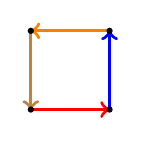
\begin{tikzpicture}[baseline=-0.5ex]
	\draw[->, red, very thick] (0,-.5) -> (1,-.5);
	\draw[->, blue, very thick] (1,-.5) -> (1,.5);
	\draw[->, orange, very thick] (1,.5) -> (0,.5);
	\draw[->, brown, very thick] (0,.5) -> (0,-.5);
	\foreach \x in {0,...,1}
	{
		\foreach \y in {-.5,...,.5}
		{
			\fill[color=black] (\x,\y) circle (.04);
		}
	}
	\end{tikzpicture}
	= \textcolor{red}{U_\mu(x)}
	\textcolor{blue}{U_\nu(x + a_\mu)}
	\textcolor{orange}{U_\mu(x + a_\nu)^\dag}
	\textcolor{brown}{U_\nu(x)^\dag}
	\]		
	\item man findet
	\[
	S_\text{Wilson} \xrightarrow{a \rightarrow 0} S_\text{YM}
	\]
\end{itemize}
\end{frame}

\begin{frame}{...in der Praxis}
	\begin{align*}
	U_\mu(x) &= 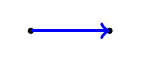
\begin{tikzpicture}[baseline=-0.5ex]
	\foreach \x in {0,1}
	{
		\foreach \y in {0}
		{
			\fill[color=black] (\x,\y) circle (.04);
		}
	}
	\draw[->, blue, very thick] (0,0) -> (1,0);
	\end{tikzpicture}, \;
	U'_\mu(x) = \begin{tikzpicture}[baseline=-0.5ex]
	\foreach \x in {0,1}
	{
		\foreach \y in {0}
		{
			\fill[color=black] (\x,\y) circle (.04);
		}
	}
	\draw[->, red, very thick] (0,0) -> (1,0);
	\draw[->, very thick] (6,0) -> (7,0) node [below] {$\mu$};
	\draw[->, very thick] (6,0) -> (6,1) node [left] {$\nu$};
	\end{tikzpicture}\\
	\rightarrow \Delta S 
	&= -\frac{\beta}{2} \sum_{\nu \neq \mu} \text{tr} \left[ \; 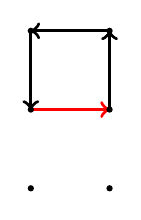
\begin{tikzpicture}[baseline=-0.5ex]
	\draw[->, very thick, red] (0,0) -> (1,0);
	\draw[->, very thick] (1,0) -> (1,1);
	\draw[->, very thick] (1,1) -> (0,1);
	\draw[->, very thick] (0,1) -> (0,0);
	\foreach \x in {0,...,1}
	{
		\foreach \y in {-1,...,1}
		{
			\fill[color=black] (\x,\y) circle (.04);
		}
	}
	\end{tikzpicture}
	\; - \;
	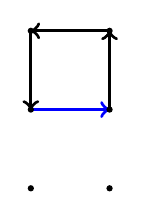
\begin{tikzpicture}[baseline=-0.5ex]
	\draw[->, very thick, blue] (0,0) -> (1,0);
	\draw[->, very thick] (1,0) -> (1,1);
	\draw[->, very thick] (1,1) -> (0,1);
	\draw[->, very thick] (0,1) -> (0,0);
	\foreach \x in {0,...,1}
	{
		\foreach \y in {-1,...,1}
		{
			\fill[color=black] (\x,\y) circle (.04);
		}
	}
	\end{tikzpicture}
	\; + \;
	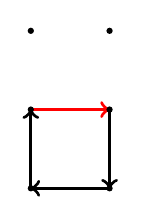
\begin{tikzpicture}[baseline=-0.5ex]
	\draw[->, very thick, red] (0,0) -> (1,0);
	\draw[->, very thick] (1,0) -> (1,-1);
	\draw[->, very thick] (1,-1) -> (0,-1);
	\draw[->, very thick] (0,-1) -> (0,0);
	\foreach \x in {0,...,1}
	{
		\foreach \y in {-1,...,1}
		{
			\fill[color=black] (\x,\y) circle (.04);
		}
	}
	\end{tikzpicture}
	\; - \;
	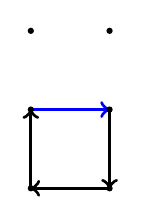
\begin{tikzpicture}[baseline=-0.5ex]
	\draw[->, very thick, blue] (0,0) -> (1,0);
	\draw[->, very thick] (1,0) -> (1,-1);
	\draw[->, very thick] (1,-1) -> (0,-1);
	\draw[->, very thick] (0,-1) -> (0,0);
	\foreach \x in {0,...,1}
	{
		\foreach \y in {-1,...,1}
		{
			\fill[color=black] (\x,\y) circle (.04);
		}
	}
	\end{tikzpicture} \; \right] \\[.5cm]
	&= -\frac{\beta}{2} \text{tr} \left[ \left( \;
	\begin{tikzpicture}[baseline=-0.5ex]
	\draw[->, very thick, red] (0,0) -> (1,0);
	\foreach \x in {0,...,1}
	{
		\foreach \y in {-1,...,1}
		{
			\fill[color=black] (\x,\y) circle (.04);
		}
	}
	\end{tikzpicture}
	\; - \;
	\begin{tikzpicture}[baseline=-0.5ex]
	\draw[->, very thick, blue] (0,0) -> (1,0);
	\foreach \x in {0,...,1}
	{
		\foreach \y in {-1,...,1}
		{
			\fill[color=black] (\x,\y) circle (.04);
		}
	}
	\end{tikzpicture}
	\; \right) \times \sum_{\nu \neq \mu} \left( \;
	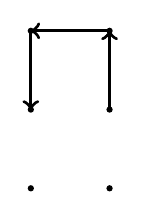
\begin{tikzpicture}[baseline=-0.5ex]
	\draw[->, very thick] (1,0) -> (1,1);
	\draw[->, very thick] (1,1) -> (0,1);
	\draw[->, very thick] (0,1) -> (0,0);
	\foreach \x in {0,...,1}
	{
		\foreach \y in {-1,...,1}
		{
			\fill[color=black] (\x,\y) circle (.04);
		}
	}
	\end{tikzpicture}
	\; + \;
	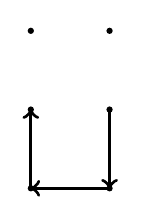
\begin{tikzpicture}[baseline=-0.5ex]
	\draw[->, very thick] (1,0) -> (1,-1);
	\draw[->, very thick] (1,-1) -> (0,-1);
	\draw[->, very thick] (0,-1) -> (0,0);
	\foreach \x in {0,...,1}
	{
		\foreach \y in {-1,...,1}
		{
			\fill[color=black] (\x,\y) circle (.04);
		}
	}
	\end{tikzpicture}
	\; \right) \right]
	\end{align*}
\end{frame}

\begin{frame}{Rekapitulierung}
	\begin{enumerate}
		\item Ziel: Berechnung von Erwartungswerten $\langle O \rangle$ mit Pfadintegralen
		\item Ansatz: Generiere Trajektorien $x^\alpha$, die nach $P^\text{Feyn}$ verteilt sind
		\item nutze den Metropolis-Algorithmus, hierfür die Wirkung $S$ des betrachteten Systems benötigt
		\item für das SU(2)-Eichfeld auf einem Gitter eignet sich $S_\text{Wilson}$.
	\end{enumerate}
\end{frame}

\begin{frame}{Wilson-Loops}
\begin{itemize}
	\item Verallgemeinerung der Plaquette \hspace{4cm} 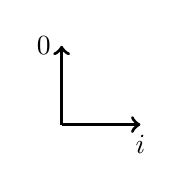
\begin{tikzpicture}
	\draw[->, very thick] (0,0) -> (1,0) node [below] {$i$};
	\draw[->, very thick] (0,0) -> (0,1) node [left] {$0$};%\in \{1,2,3\}$};
	\end{tikzpicture}
	\[
	W(3,2) = \text{tr} \left[ \; 	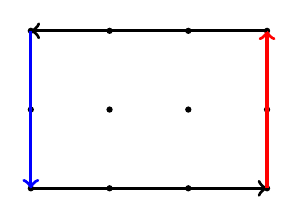
\begin{tikzpicture}[baseline=-0.5ex]
	\foreach \x in {0,...,3}
	{
		\foreach \y in {-1,...,1}
		{
			\fill[color=black] (\x,\y) circle (.04);
		}
	}
	\draw[->, black, very thick] (0,-1) -> (3,-1);
	\draw[->, red,   very thick] (3,-1) -> (3,1);
	\draw[->, black, very thick] (3,1) -> (0,1);
	\draw[->, blue,  very thick] (0,1) -> (0,-1);
	\end{tikzpicture}
	\; \right]
	\]
	\item Erwartungswert (Beweis s. Rothe~\cite{loopsStaticPotRothe})
	\[
	\langle W(r,t) \rangle \xrightarrow{t \rightarrow \infty} A \cdot e^{-t V(r)}.
	\]
\end{itemize}
\end{frame}

\section{Implementierung}

\begin{frame}{SU(2)-Matrizen}
\begin{itemize}
	\item Eigenschaften von Elementen $U \in SU(2)$:
	\[
	U \in \mathds{C}^{2 \times 2}, U^\dag U = U U^\dag = \mathds{1}, \text{det} \, U = 1
	\]
	\item Darstellung nach Urbach \& Petschlies~\cite{urbachCPscript}:
	\[
	U =
	\begin{pmatrix}
	a    & b   \\
	-b^* & a^* \\
	\end{pmatrix},
	\; a, b \in \mathds{C}, \; |a|^2 + |b|^2 = 1.
	\]
	\item Zufallsgenerierung über Isomorphismus
	\begin{align*}
	\phi: S^3 &\rightarrow \mathrm{SU}(2),\\
	(x^0, \vec{x}) &\mapsto x^0 \mathds{1} + i \vec{x} \cdot \vec{\sigma},
	\end{align*}
	\vspace{-1.4cm}
\begin{multicols}{2}
	\[
	\rightarrow \begin{pmatrix}
	x^0 \\
	x^1 \\
	x^2 \\
	x^3
	\end{pmatrix}
	=
	\begin{pmatrix}
	\cos(\chi) \sin(\vartheta) \cos(\varphi) \\
	\sin(\chi) \sin(\vartheta) \cos(\varphi) \\
	\sin(\chi) \sin(\vartheta) \sin(\varphi) \\
	\sin(\chi) \cos(\vartheta)
	\end{pmatrix},
	\]
	\break
	\vspace{-1cm}
	\begin{align*}
	\chi &\in (0, 2 \pi \cdot \delta),\\
	\varphi &\in (0, 2 \pi),\\
	\cos(\vartheta) &\in (-1,1).
	\end{align*}
\end{multicols}
\end{itemize}
\end{frame}

\begin{frame}{Rekapitulierung}
	\begin{enumerate}
		\item Ziel: Berechnung von Erwartungswerten $\langle O \rangle$ mit Pfadintegralen
		\item Ansatz: Generiere Trajektorien $x^\alpha$, die nach $P^\text{Feyn}$ verteilt sind
		\item nutze den Metropolis-Algorithmus, hierfür die Wirkung $S$ des betrachteten Systems benötigt
		\item für das SU(2)-Eichfeld auf einem Gitter eignet sich $S_\text{Wilson}$ (unter Verwendung der Paralleltransporte $U_\mu(x)$).
		\item Untersuchung des statischen Potentials mit Wilson-Loops als Observable:
		\[
		\langle W(r,t) \rangle \xrightarrow{t \rightarrow \infty} A \cdot e^{-t V(r)}.
		\]
	\end{enumerate}
\end{frame}

\begin{frame}[fragile]{Exemplarische \texttt{main}-Funktion}
	\begin{lstlisting}[language=C++,basicstyle=\small]
int main() {
  ...
  for (std::size_t i=0; i < 1000; i++) {
    sweep(U, beta, delta, iterationsPerSight, engine);
  }
  ...
  for (std::size_t i=0; i < 20000; i++) {
    results.push_back(getSqrt2Loop(U, 2));
	
    for (size_t j = 0; j < 5; j++) {
        sweep(U, beta, delta, iterationsPerSight, engine);
      }
  }
  ...
  return 0;
}
	\end{lstlisting}
\end{frame}

\section{Messergebnisse}

\begin{frame}{Einzelne Messungen}
	\centering
    \includegraphics[width=.8\textwidth]{1x3loop}
\end{frame}

\begin{frame}{Verteilung der Messwerte}
	\centering
	\includegraphics[width=.8\textwidth]{1x3and4histogramPresentation}
\end{frame}

\begin{frame}{Extrahierung des statischen Potentials (i)}
	\centering
	\includegraphics[width=.8\textwidth]{loopResultsBeta23r3.pdf}
\end{frame}

\begin{frame}{Extrahierung des statischen Potentials (ii)}
\begin{figure}
    \centering
	\includegraphics[width=.6\textwidth]{aVfitBeta23.pdf}
	\begin{minipage}[b]{.35\textwidth}
		Modell:
		\[
		a V(r) = -\frac{A}{r} + B + \sigma \cdot r
		\]
		Ergebnis:
		\begin{align*}
		A &= (0.277 \pm 0.024) a\\
		B &= (0.524 \pm 0.034) \\
		\sigma &= (0.189\pm 0.010) \frac{1}{a}
		\end{align*}
	\end{minipage}
\end{figure}
\end{frame}

\section{Ausblick}

\begin{frame}{Was gibt es als Nächstes zu tun?}
\begin{itemize}
	\item Fehlerbetrachtung verbessern
	\item wirklich der Grundzustand? $\rightarrow$ größere Gitter vermessen, effektive Masse betrachten
%	\item Phasenübergang untersuchen
	\item SU(3) untersuchen
\end{itemize}
\end{frame}

\begin{frame}{Literatur}
\printbibliography
\end{frame}
  
\end{document}